\clearpage{\pagestyle{empty}\cleardoublepage}

\chapter{Microscopia a fluorescenza}

\begin{flushright}\begin{small}\textit{"Man is the interpreter of nature,\\ 
science the right interpretation."}\\
- William Whewell -\\
\end{small}\end{flushright}

Questo capitolo si propone di descrivere un tipico microscopio a fluorescenza, ponendo in particolare l'attenzione sul microscopio Nikon Eclipse-Ti, e inoltre di esaminare le principali imperfezioni e difetti presenti nelle immagini con esso acquisite.

\section {Il microscopio a fluorescenza}

Il microscopio a fluorescenza permette di studiare campioni organici o inorganici sfruttando i fenomeni di luminescenza descritti nel precedente capitolo, piuttosto che quelli di riflessione ed assorbimento della luce, basilari invece per i microscopi ottici tradizionali. 
In genere tale strumento è in grado di funzionare anche come microscopio ottico convenzionale, permettendo così il confronto tra le immagini acquisite nelle due diverse modalità.

Questo tipo di microscopia è caratterizzata dalla marcatura specifica del target in esame con una sonda fluorescente (capitolo 1.3.1) e da una struttura base dello strumento, costituita da: sorgente di luce, filtri, obiettivo e sistema di rivelazione. 
La descrizione che segue fa riferimento ad un microscopio a fluorescenza rovesciato (\figurename~\ref{fig:micro}), ove l'ottica è posizionata al di sotto del tavolino porta oggetti. 
Tale scelta è stata fatta per poter comprendere più facilmente il funzionamento del microscopio Nikon Eclipse-Ti che verrà analizzato successivamente.

\begin{figure}
 \centering
 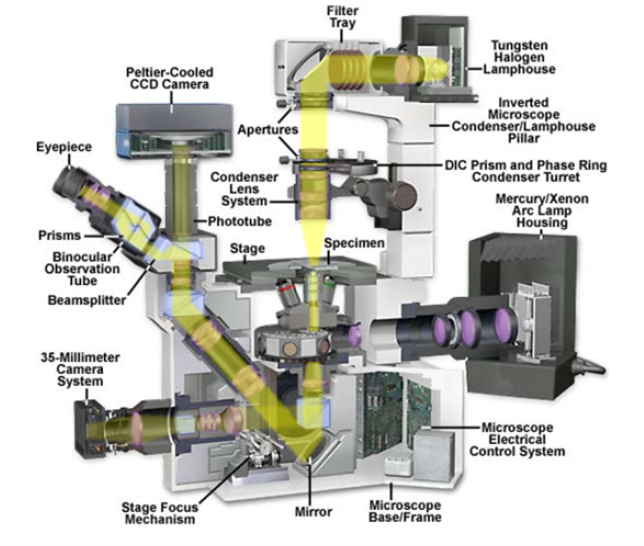
\includegraphics[scale=.60]{img/CAP2microrovesciato.jpg}
 \caption{\small{Schema ottico di un microscopio a fluorescenza rovesciato.}}
 \label{fig:micro}
\end{figure}

La sorgente di luce deve essere scelta in modo da massimizzare la quantità di fluoroforo eccitato, quindi l'intensità di emissione. 
Per questo motivo le lampade ad incandescenza non sono adatte, in quanto emettono prevalentemente luce di incandescenza nel rosso e nell'IR, con grande dispersione di calore. 
La scelta ricade in genere sulle \textbf{lampade a globo di quarzo} contenenti vapori di mercurio ad alta pressione, che soddisfano tutte le condizioni richieste. 

Esse vengono denominate con le sigle HBO 50 o HBO 100 a seconda della potenza dissipata e, a differenza delle lampade ad incandescenza, sfruttano il fenomeno delle scariche dei gas, caratteristica che gli conferisce uno spettro discreto. 
Questa lampada è costituita da un globo di quarzo, resistente alle alte pressioni, in cui sono fusi due elettrodi. 
Nella camera di combustione interna, contenente mercurio, viene generato e mantenuto attivo un arco voltaico tramite scariche ad alta tensione applicate agli elettrodi; il calore prodotto fa evaporare il mercurio, così da creare una situazione di sovrapressione. 

La lampada in esame emette luce molto intensa nello spettro UV, mentre nella parte del visibile l'intensità è più bassa, ma comunque sfruttabile per altre applicazioni. 
I picchi di intensità risultano proprio in corrispondenza dei cosiddetti ``picchi del mercurio'' (\figurename~\ref{fig:lamp}).

\begin{figure}
 \centering
 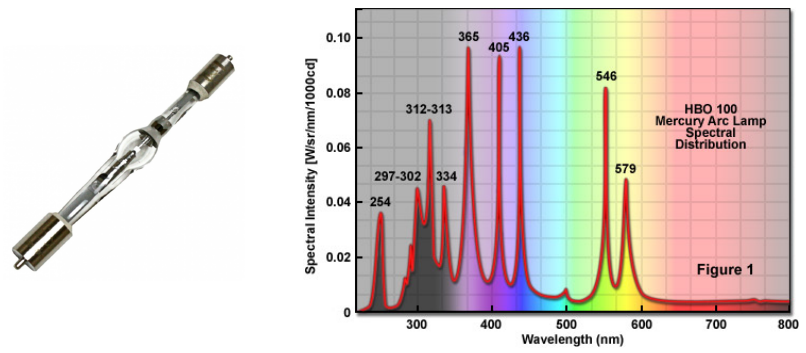
\includegraphics[scale=.48]{img/CAP2lampadaquarzo.png}
 \caption{\small{Arc-discharge fluorescence mercury lamp HBO 100 (sinistra) con associato spettro di emissione (destra).}}
 \label{fig:lamp}
\end{figure}

Come visto nel capitolo 1.3, il fascio di luce che raggiunge il campione deve avere una lunghezza d'onda prossima al picco di eccitazione del fluoroforo e inoltre il microscopio deve essere in grado di rivelare selettivamente la lunghezza d'onda di emissione di tale molecola, generando quindi un alto contrasto tra il background e le strutture fluorescenti.
Per soddisfare al meglio queste due richieste si sfruttano due filtri:
\begin{description}
\item[Filtro di eccitazione:]
Serve per filtrare la luce proveniente dalla sorgente prima che raggiunga il campione, lasciando passare così solo la lunghezza d'onda necessaria per l'eccitazione.
\item[Filtro barriera o di sbarramento:]
Serve per filtrare la luce proveniente dal campione, bloccando così la radiazione di illuminazione non assorbita dal fluoroforo e lasciando quindi passare solo quella di emissione. 
\end{description}
Per poter capire il loro utilizzo, servendoci della \figurename~\ref{fig:micro}, ripercorriamo il cammino ottico della luce di eccitazione: la luce emessa dalla lampada al mercurio passa attraverso l'illuminatore lungo un asse perpendicolare all'asse ottico primario del microscopio, attraversando una lente collettrice e un diaframma di apertura e centratura variabile. 
La luce viene poi filtrata dal filtro di eccitazione e incontra successivamente uno \textbf{specchio dicroico} (chromatic beamsplitter). 
Quest'ultimo è un filtro interferenziale specializzato nel riflettere le piccole lunghezze d'onda e trasmettere quelle più alte; esso è posto su in piano inclinato a 45° rispetto alla direzione della luce incidente e riflette la luce a 90° rispetto alla stessa direzione, proiettandola attraverso l'obiettivo, sino a colpire il campione. 
Il segnale di fluorescenza emesso dal campione viene quindi raccolto dal medesimo obiettivo e passa attraverso lo specchio dicroico, in virtù del fatto che la sua lunghezza d'onda risulta maggiore di quella di eccitazione, per lo shift di Stokes. 
Questo segnale di emissione passa attraverso il filtro di sbarramento e infine raggiunge i dispositivi per la formazione dell'immagine.

Spesso i filtri e lo specchio dicroico vengono montati in un unico blocco ottico detto \textit{filter cube} (\figurename~\ref{fig:cube}). 
Notiamo quindi che è proprio in base a tali elementi che si stabilisce quali molecole fluorescenti usare, infatti è possibile sfruttare unicamente quei fluorofori con lunghezze di eccitazione e di emissione corrispondenti a quelle trasmesse dai filtri. 
Inoltre, combinando vari filtri è possibile l'osservazione di un gran numero di fluorocromi con differenti proprietà di eccitazione ed emissive.

\begin{figure}
 \centering
 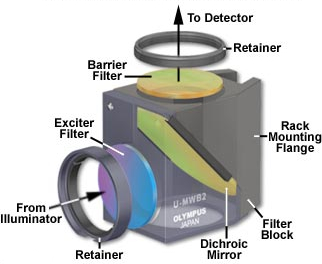
\includegraphics[scale=.65]{img/CAP2cube.jpg}
 \caption{\small{Schema ottico di un filter cube per microscopi a fluorescenza rovesciati.}}
 \label{fig:cube}
\end{figure}

Altro elemento fondamentale è certamente l'\textbf{obiettivo} e, come accennato, le sue lenti svolgono una duplice funzione: focalizzazione della luce di eccitazione sul campione (ancor più rispetto al sistema di lenti del condensatore presente in un microscopio convenzionale) e raccolta della luce di fluorescenza emessa. 

Gli obiettivi possono essere di diverso tipo e sono caratterizzati dalle informazioni riportate su di essi, come per esempio: fabbricante, ingrandimento ($4x,\ 10x,\ 20x,\ 40x,\ 60x\ o\ 100x$), requisiti per l'immersione ad aria, olio o acqua (in genere obiettivi con ingrandimento minore di $40x$ sono ad aria e quelli con ingrandimento pari o superiore a $40x$ sono ad immersione) e spessore del vetrino coprioggetti (solitamente $0.17\ mm$).  
Possono essere riportate anche informazioni relative alle correzioni per artefatti ottici, come aberrazioni cromatiche e appiattimento di campo.
Ne sono degli esempi le scritte ``fluo'' per lenti meno corrette o ``plan'' e ``plan apo'' per lenti con correzioni più fini. 

Altro parametro sempre presente sull'obiettivo è l'apertura numerica ($NA$, Numerical Aperture). 
Essa è una misura della capacità di una lente di raccogliere la luce del campione ed è definita dalla relazione:
$$ NA = n \cdot sin \theta $$
dove $n$ è l'indice di rifrazione del mezzo presente tra lente e campione e $\theta$ è l'apertura angolare della lente, ossia il semiangolo del cono di luce che entra nell'ottica. 
Il range di variabilità della $NA$ è solitamente tra 0.25, per obiettivi a basso ingrandimento e a secco (es. $10x$), e 1.45, per obiettivi ad immersione (es. da $40x$ a $100x$). 
In microscopia a fluorescenza è necessario utilizzare obiettivi con alta apertura numerica, così da massimizzare la quantità di luce raccolta dal campione \cite{NA}.
Infatti, la luminosità L dell'immagine, definita come flusso di fotoni per unità di superficie e di tempo ($W/m^2$), è legata all'apertura numerica tramite la relazione:
$$L  \propto  \frac {NA^4}{I^2}$$
dove $I$ è l'ingrandimento. 
Risulta quindi evidente che le immagini a fluorescenza più brillanti saranno raccolte da obiettivi con grande $NA$ e piccolo $I$; dei buoni valori sono per esempio $NA=0.75$ e $I=20x$.
D'altra parte il guadagno ottenuto aumentando l'apertura numerica, molto utile dato che le emissioni in fluorescenza risultano decisamente poco intense, comporta alcuni effetti indesiderati, come l'aumento dell'autofluorescenza e delle riflessioni da parte delle superfici delle lenti interne che riducono l'intensità finale. 
Tale problema può essere in parte marginato usando un liquido d'immersione, specialmente olio, così da eliminare la perdita di luce
causata dai riflessi sulle superfici e rendere l'immagine più chiara. 
Inoltre, una maggior apertura numerica migliora anche la risoluzione $d$ dell'immagine, poiché data dall'equazione:
$$d = 0.61 \ \frac {\lambda}{NA} $$
dove $\lambda$ è la lunghezza d'onda della luce di eccitazione.

Come visto precedentemente, nei microscopi a fluorescenza l'illuminazione è pensata in modo tale che sia la luce di eccitazione che quella di emissione passino per lo stesso obiettivo: ciò comporta numerosi vantaggi. 
Innanzitutto il fatto che l'obiettivo funzioni sia da condensatore che da dispositivo di formazione dell'immagine fa sì che l'allineamento condensatore-obiettivo sia sempre perfetto, che l'area illuminata dalla luce di eccitazione sia ristretta a quella che si osserva attraverso l'obiettivo e che sia disponibile tutta l'apertura numerica dell'obiettivo stesso; infine questa configurazione permette di combinare la tecnica della fluorescenza con alcune tecniche in luce trasmessa.


\subsection{Microscopio Nikon Eclipse-Ti}

Il microscopio a fluorescenza rovesciato Nikon Eclipse-Ti è stato acquistato alcuni anni fa dal Dipartimento di Fisica di Bologna per lo studio biofisico di alcuni effetti prodotti da radiazioni ionizzanti su cellule di fibroblasti umani, nell'ambito della ricerca sperimentale sull'invecchiamento fisiologico ed indotto dall'esposizione a radiazioni ionizzanti a differenti dosi. 

Tale microscopio può essere utilizzato sia per la microscopia in fluorescenza, sia per quella in campo chiaro a luce trasmessa.
Per poter rivelare la luce emessa dal campione è possibile sfruttare sia l'oculare che un sistema di rivelazione digitale, come per esempio una telecamera.
Nel caso in cui si utilizzi quest'ultimo sistema di rivelazione, le immagini verranno visualizzate sul monitor di un computer e registrate in formato digitale grazie ad appositi softwares, tramite cui è anche possibile elaborare ed analizzare le acquisizioni. 
La scelta di registrare le immagini rende inoltre possibile confrontare situazioni a tempi diversi e quindi creare una misura in dinamica, cosiddetta ``time-lapse''. 
La caratteristica principale di tale strumento è la possibilità di fare acquisizioni in vivo in time-lapse, anche per decine di ore, grazie ad un innovativo sistema di incubazione, in grado di mantenere in vita le cellule, integrato con il tavolino portaoggetti motorizzato ed un sistema di ``perfect focus''.

\begin{figure}
 \centering
 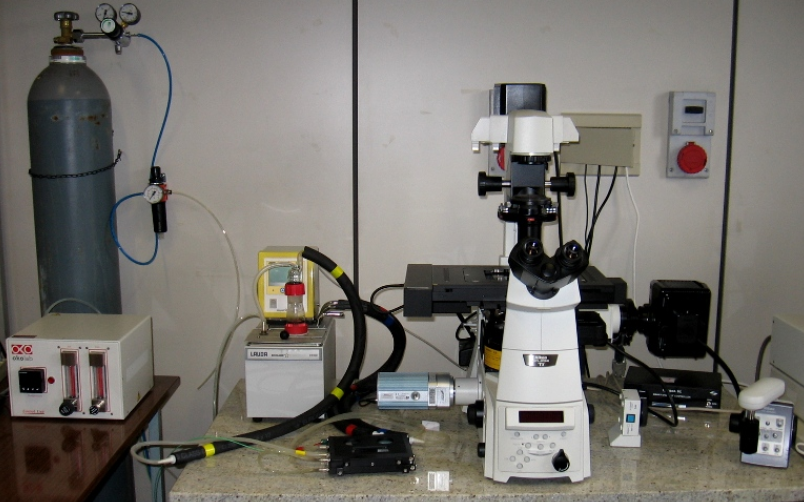
\includegraphics[scale=.45]{img/CAP2microNIKON.png}
 \caption{\small{Microscopio Nikon Eclipse-Ti.}}
 \label{fig:NIKON}
\end{figure}

Qui di seguito viene riportata una descrizione dei vari elementi che compongono il microscopio Nikon Eclipse-Ti (\figurename~\ref{fig:NIKON}):

\begin{description}

\item[Lampada diascopica:]
\'E una lampada alogena (TI-DH Dia Pillar Illuminator 12V/100W) per osservazioni in campo chiaro e contrasto di fase.

\item[Lampada episcopica:]
Si tratta di una lampada per la fluorescenza al mercurio HBO (arc-discharge fluorescence mercury lamp HBO) analoga a quelle descritte in precedenza.

\item[Obiettivi:]
Gli obiettivi disponibili sono $10x$, $20x\ Fluo$, $40x\ Super\ Fluo$, $60x\ Oil\ Fluo$ e rispettano, seppur con qualche compromesso, le esigenze sia dell'imaging cellulare in dinamica che dell'imaging in fluorescenza. 
Scegliere il giusto obiettivo è molto importante ai fini di un maggior segnale dal campione ed un miglior trasferimento di esso al sistema di rivelazione.

\item[Smart Shutter ultraveloce LAMBDA SC:]
Esso permette di decidere quando lasciare che la luce illumini il campione e quando no, senza dover spegnere manualmente la lampada sorgente.
Tramite software si può inoltre programmare ogni quanto aprire e chiudere lo shutter.

\item[Filter Cube:]
Questo microscopio è dotato di un meccanismo scorrevole che può contenere fino a sei cubi, così da disporre velocemente di sei combinazioni di filtri diversi \cite{Nikon1}. 
Attualmente dispone di 3 cubi, che permettono combinazioni di filtri per l'osservazione di fluorofori che emettono nel blu, nel rosso e nel verde, con eccitazioni tipiche dei coloranti più diffusi, che sono rispettivamente: DAPI, TRITC e FITC. 
I filtri sono denominati in associazione a tali fluorocromi, tuttavia presentano configurazioni di eccitazione e di emissione molto versatili, in quanto esiste un grande numero di fluorofori con proprietà compatibili con esse. 
In \tablename~\ref{TAB} sono riportate le bande di eccitazione e di emissione dei cubi a disposizione:

\begin{table}[!ht]
 \begin{center}
\begin{small}
\begin{tabular}{lccc}
\hline\hline
&\textbf{$\lambda$ eccitazione (nm)}&\textbf{$\lambda$ emissione (nm)}&\textbf{$\lambda$ dicroico (nm)}\\
\hline
\textbf{DAPI}&330 - 380&$\geq$ 420&400\\
\textbf{TRITC}&515 - 565&550 - 660&565\\
\textbf{FITC}&465 - 495&515 - 555&505\\
\hline\hline
\end{tabular}
\caption{\small{Bande dei tre filter cubes del Nikon Eclipse-Ti del Dipartimento di Fisica di Bologna.}}
\label{TAB}
\end{small}
\end{center}
\end{table}

\item[Telecamera:]

\begin{figure}
 \centering
 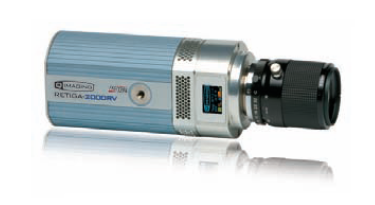
\includegraphics[scale=.60]{img/CAP2CCD.png}
 \caption{\small{Telecamera Qimaging, modello RETIGA-2000-RV.}}
 \label{fig:CCD}
\end{figure}

Il rivelatore CCD di cui è dotato il microscopio è una telecamera Qimaging, modello RETIGA-2000-RV (\figurename~\ref{fig:CCD}), in grado di rilevare segnali di bassa intensità, con un alto range dinamico e applicazioni rapide, caratteristiche che la rendono particolarmente adatta per l'imaging dinamico in vivo e in fluorescenza.
La telecamera presenta un sistema di raffreddamento che permette di regolare la temperatura fino a 30°C sotto zero, così da ridurre drasticamente il rumore termico, che costituisce un grande problema in quanto riduce il rapporto segnale-rumore nell'imaging dinamico.
Essa è sincronizzata con le lampade di illuminazione del microscopio, con il tavolino motorizzato, con il filter cube e lo shutter. 
Il rivelatore CCD ha 1.92 megapixel e produce un output a 12 bit in livelli di grigio.
È dotata di un filtro IR (infrarosso), posto di fronte al rivelatore, necessario per abbattere la componente IR che potrebbe provenire dal sistema di rilevamento del fuoco (Perfect Focus System). 
Infine, il tempo di esposizione può variare entro il range $10\ \mu s - 17.9\ min $, regolabile attraverso software.

\item[Sistema di incubazione:]
Il microscopio Nikon Eclipse-Ti è dotato di un supporto per il tavolino portaoggetti, adatto all'inserimento di un piccolo incubatore fabbricato dalla ditta Oko-Lab (\figurename~\ref{fig:okolab} e \figurename~\ref{fig:controllo}).
Al suo interno si crea un ambiente adatto alla sopravvivenza delle cellule, con una temperatura controllata, una miscela di aria e anidride carbonica fornita tramite bombola ed un certo tasso di umidità gestito da un apposito bagno termostatato.

\begin{figure}
 \centering
 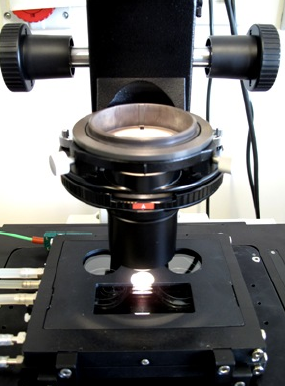
\includegraphics[scale=.60]{img/CAP2okolab.png}
 \caption{\small{Incubatore della Oko-Lab integrato con il tavolino portaoggetti del microscopio Nikon Eclipse-Ti.}}
 \label{fig:okolab}
\end{figure}

\begin{figure}
 \centering
 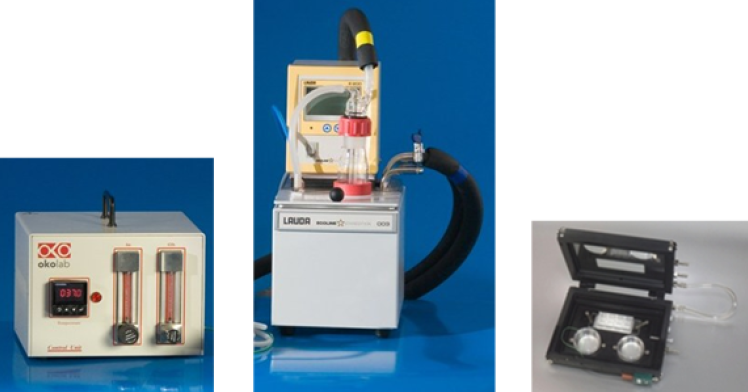
\includegraphics[scale=.45]{img/CAP2controllo.png}
 \caption{\small{Sistemi di controllo dell'aria e della $CO_2$ (sinistra), termostato a bagno termico (centrale) ed incubatore della Okolab (destra).}}
 \label{fig:controllo}
\end{figure}

Per creare e mantenere questo microclima all'interno dell'incubatore sono necessari diversi sistemi di controllo (\figurename~\ref{fig:controllo}). 
La temperatura è regolata attraverso un apposito software che la rileva costantemente sfruttando una termocoppia collegata all'unità di controllo. 
Essa è mantenuta costante grazie ad un termostato a bagno termico che tramite una resistenza scalda l'acqua, la inietta in un'intercapedine e, scorrendo lungo i bordi del piccolo incubatore, scalda l'aria al suo interno.
La stessa unità di controllo che regola la temperatura, se collegata ad una pompa ad aria compressa e ad una bombola di $CO_2$, permette all'operatore di regolare il flusso di aria ed anidride carbonica, creando in tal modo l'``atmosfera'' ideale per la vitalità delle cellule.
Infine, per quanto riguarda l'umidità è presente un'unità apposita, immersa nel bagno termico, in grado di produrre del vapore, successivamente immesso all'interno dell'incubatore.

\item[Perfect Focus System (PFS):]
Il PFS è un meccanismo hardware ideato dalla Nikon per poter contrastare gli spostamenti assiali del tavolino motorizzato ed evitare in tal modo la perdita del fuoco (vedere la sezione \ref{PFS}).

\item[Software Nis-Element 3.1:]
Esso è il software attraverso cui si gestiscono le varie funzionalità del microscopio, dalla creazione di sequenze di acquisizione spazio-temporali sino all'analisi delle immagini ottenute (vedere la sezione \ref{NisElements}).

\end{description}


\subsection{Perfect Focus System (PFS)}\label{PFS}

Supponendo che tutte le condizioni ambientali esterne al campione siano ideali, l'unico disturbo alla misura è la perdita intrinseca del fuoco dovuta ai gradienti termici, vibrazioni, instabilità meccaniche e un certo numero di altri fattori difficilmente eliminabili.

La Nikon ha affrontato questo problema progettando una soluzione hardware, detta \textit{Perfect Focus System} (PFS), pensata per contrastare gli spostamenti assiali in tempo reale nell'arco dell'intera acquisizione \cite{Nikon2}. 
Tale soluzione risulta molto utile specialmente negli esperimenti in cui si osservano più parti del campione, ove gli spostamenti macroscopici del tavolino motorizzato sono inevitabili.

\begin{figure}
 \centering
 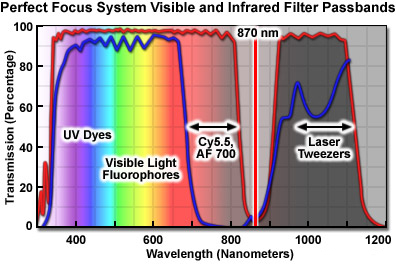
\includegraphics[scale=.65]{img/CAP2bande.png}
 \caption{\small{Bande di emissione dei marcatori fluorescenti e del LED a 870 nm.}}
 \label{fig:bande}
\end{figure}

Punto critico del PFS è il rilevamento accurato di un certo piano assiale che possa essere utilizzato come riferimento per stabilire con precisione la distanza che deve intercorrere tra la superficie della lente obiettivo ed il piano focale di interesse nel campione. 
A questo scopo il PFS utilizza un LED infrarosso a $870\ nm$ che non interferisce con i segnali raccolti dall'ottica dell'obiettivo: nè con la luce di eccitazione, né con quella emessa dai fluorofori, poiché presentano lunghezze d'onda di emissione comprese entro il range $[340\ -\ 770]\ nm$ (\figurename~\ref{fig:bande}).

\begin{figure}
 \centering
 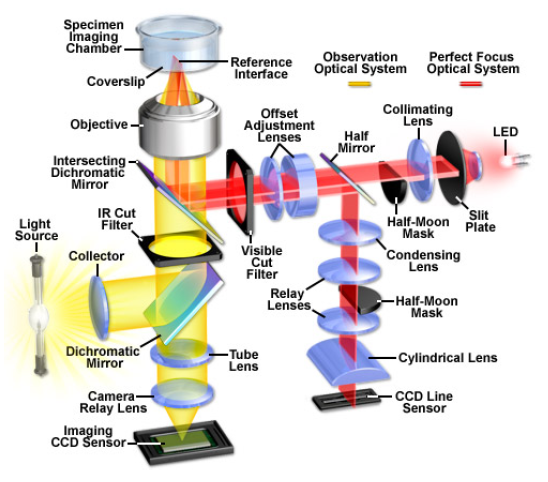
\includegraphics[scale=.70]{img/CAP2PFSschema.png}
 \caption{\small{Schema ottico dell'unità di Perfect Focus System (PFS).}}
 \label{fig:PFSschema}
\end{figure}

Servendoci della \figurename~\ref{fig:PFSschema} ripercorriamo il percorso della luce prodotta dal LED. 
Innanzitutto viene fatta passare attraverso una lente condensatrice e la fenditura di una piastrina (Slit Plate).
Una lente collimatrice converte la luce in un fascio di raggi paralleli, fatti passare poi in una maschera a mezza luna (half-moon mask), che serve per abbattere una parte dei raggi luminosi lungo l'asse ottico.
Il fascio viene quindi trasmesso all'half-mirror, focalizzato dalle lenti del sistema di regolazione dell'offset e diretto verso un filtro anteposto all'ingresso del percorso ottico primario. 
L'ingresso a tale percorso è mediato dallo specchio dicroico, che funge da intersezione dei due sistemi ottici trasmettendo la luce visibile e riflettendo quella infrarossa, evitando così che luce trasmessa o segnale di fluorescenza siano contaminati dal PFS. 
A questo punto, il fascio originato dal LED viene focalizzato dall'obiettivo sull'interfaccia di riferimento, ossia sulla superficie ove l'indice di rifrazione cambia: o da coprivetrino ($n=1.5$) ad aria ($n=1$) o da coprivetrino a mezzo che circonda il campione ($1.33\leq n \geq 1.38$), rispettivamente per obiettivi a secco e ad immersione. 
Su tale interfaccia la luce viene nuovamente riflessa e convertita in una fascio di raggi paralleli nel sistema ottico primario. 
Quindi lo specchio dicroico riflette ancora il fascio, permettendone il rientro nel sistema ottico del PFS.
Passano di nuovo attraverso il filtro per la luce visibile e le lenti di regolazione dell'offset, per poi entrare nell'half-mirror e quindi nel nuovo percorso in cui si forma l'immagine di rilevamento del fuoco. 
Qui il fascio viene ritrasformato nell'immagine della fenditura da una lente collettrice, fatto passare attraverso le lenti ritardanti, la maschera a mezza luna ed una lente cilindrica per poi arrivare nella parte centrale del sensore CCD lineare sotto forma di una linea marcata.

Una componente molto importante del PFS è il sistema di lenti per la regolazione dell'offset, posta tra l'half-mirror e lo specchio dicroico.
Esso produce uno shift della posizione a fuoco dell'immagine della fenditura, in coordinazione con un sistema elettronico di feedback che controlla la posizione assiale del tavolino motorizzato.

\begin{figure}
 \centering
 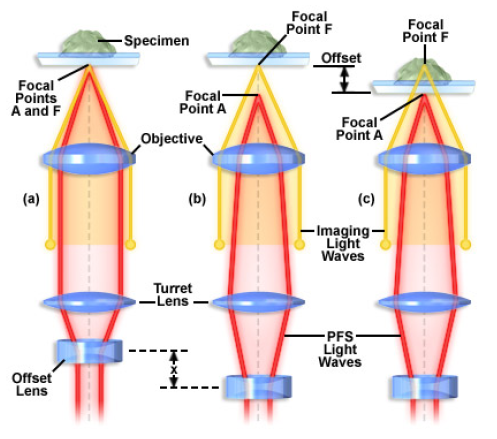
\includegraphics[scale=.65]{img/CAP2PFS.png}
 \caption{\small{Regolazione dell'offset nel PFS.}}
 \label{fig:PFS}
\end{figure}

La \figurename~\ref{fig:PFS} mostra come l'immagine del piano focale del campione (raggio giallo) e quella della fenditura (raggio rosso) siano rispettivamente dirette verso il rivelatore (o l'oculare) e verso il sensore CCD lineare attraverso due percorsi ottici indipendenti.
L'immagine fa riferimento al caso particolare di obiettivi a secco, ossia ad interfaccia di riferimento data da coprivetrino-aria.
Si nota che le lenti di offset si spostano in modo da regolare la posizione dell'immagine della fenditura sul sensore, mentre la ``lente torretta'' è fissa sull'asse ottico. 
Inoltre, prima dell'inizializzazione del PFS, si ha una condizione di offset nullo, ossia la posizione di fuoco della lente obiettivo (F) e dell'immagine della fenditura (A) coincidono all'interfaccia di riferimento (\figurename~\ref{fig:PFS}/a). 
Per poter introdurre un offset tra i piani focali delle due immagini si può variare la posizione della lente di offset attraverso una manopola del PSF, e quindi variare anche la posizione di fuoco dell'immagine di fenditura (\figurename~\ref{fig:PFS}/b). 
Quando poi il sistema di feedback del PFS regola la $z$ dell'obiettivo in modo da ristabilire il piano focale A all'interfaccia coprivetrino-aria, il piano focale dell'immagine F viene spostato nella parte centrale del campione in esame (\figurename~\ref{fig:PFS}/c). 
La distanza di offset che ora separa i due piani focali può essere regolata dall'operatore in modo da esplorare diversi piani di fuoco all'interno del campione.
Quando l'interfaccia di riferimento si sposta lungo l'asse z l'immagine della fenditura sul rivelatore risulta shiftata e sfuocata e di conseguenza il controller del PFS sposta l'obiettivo in direzione compensatoria al movimento precedente fin quando non raggiunge nuovamente la situazione in cui l'immagine della fenditura compare al centro del sensore. 

Tale sistema di controllo del fuoco presenta come vantaggio più grande il fatto di essere più veloce di ogni altro sistema esistente, in quanto il feedback viene fornito dal PFS ogni $5\ ms$ (per altri meccanismi esistenti di mantenimento del fuoco viene fornito al più ogni $500\ ms$) e la distanza tra l'obiettivo e il campione viene mantenuta costante con una precisione assiale di $0.025\ nm$. 
Tuttavia il PFS presenta alcuni limiti di utilizzo, legati al tipo di campione e di supporto usati. 
Per esempio, nel caso di campioni immersi in mezzi acquosi occorre che lo spessore del mezzo sia di almeno $3\ mm$; la camera su cui sono coltivati i campioni deve avere un fondo di spessore compreso tra $150\ nm$ e $180\ nm$ per permettere una riflessione ottimale del segnale infrarosso; campioni troppo spessi o seminati su petri o vetrini di materiali diversi dal vetro, come per esempio la plastica, che presentano un forte scattering dell'infrarosso, non sono adatti per l'utilizzo del PFS. 

Infine bisogna osservare che l''unità PFS Nikon è situata nel gruppo ottico di sei obiettivi, situato tra la torretta dei filtri per la fluorescenza e il tavolino del microscopio; che i suoi controlli elettronici sono anch'essi all'interno del gruppo ottico e sono autosufficienti, cioè non richiedono un software supplementare per la loro gestione e che il PFS può essere attivato o disattivato tramite una leva che inserisce o meno lo specchio dicroico nel percorso ottico primario del microscopio.


\subsection{Software: Nis-Element 3.1}\label{NisElements}

Nis-Element 3.1 è, come accennato, il software associato al microscopio Nikon Eclipse-Ti.
Tramite tale software le immagini possono essere osservate o in modalità ``live'', ovvero in tempo reale, oppure in modalità di ``visualizzazione'', cioè mostrando le immagini acquisite e salvate in precedenza, su cui è possibile avviare un'eventuale elaborazione attraverso gli strumenti di analisi delle immagini digitali di cui il programma dispone.

\begin{figure}
 \centering
 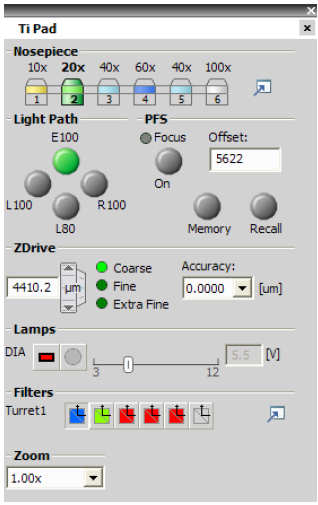
\includegraphics[scale=.50]{img/CAP2pannello.png}
 \caption{\small{Microscope Control Pad (Tipad).}}
 \label{fig:pannello}
\end{figure}

Nella schermata iniziale è presente un riquadro che visualizza l'immagine in esame ed il pannello ``Microscope Control Pad'', detto anche TiPad (\figurename~\ref{fig:pannello}), da cui l'utente può gestire i diversi componenti del microscopio. 
Tale pannello dispone delle seguenti sezioni di controllo:

\begin{description}
\item[Nosepiece:]
Permette la selezione dell'obiettivo da utilizzare durante l'osservazione e crea differenti configurazioni ottiche a seconda dell'obiettivo montato dall'utente sul corpo ottico del microscopio.

\item[Light Path:]
Questa box riproduce la stessa pulsantiera a croce presente alla base del microscopio (\figurename~\ref{fig:NIKON}), attraverso cui si seleziona il percorso ottico della luce. 
Le due modalità ``L100'' e ``R100'' mandano il 100\% del segnale rispettivamente all'uscita di sinistra e di destra, dove sono presenti i collegamenti per i rivelatori CCD; la modalità ``Eye'' direziona tutto il segnale verso l'oculare; la modalità ``L80'' direziona l'80\% del segnale verso l'uscita del rivelatore di sinistra ed il 20\% verso l'oculare.

\item[PFS:]
\'E il pulsante per l'attivazione e la disattivazione del Perfect Focus System. 
Quando la spia è verde significa che il PFS è attivato ed il fuoco non è più regolabile con la manopola tradizionale ma con quella del PFS. 
Una volta messa a fuoco l'immagine, cliccando sul pulsante Memory si può memorizzare l'offset della posizione scelta.

\item[Z Drive:]
Permette di decidere la sensibilità degli spostamenti assiali del tavolino motorizzato per la ricerca del piano focale nella modalità senza PFS inserito.
\'E possibile impostare tre differenti sensibilità: Coarse (grezzo), Fine (fine) e ExFine (extra fine).

\item[Lamp:]
Questa box permette l'accensione e la regolazione della potenza della luce di illuminazione per le osservazioni in luce trasmessa.

\item[Filters:]
Questa box permette di inserire nel percorso ottico primario del microscopio i diversi filter cubes necessari per la fluorescenza.
L'operatore può creare configurazioni differenti a seconda delle combinazioni di filtri di cui dispone, memorizzando per ciascuna le bande di lunghezze d'onda del filtro di eccitazione, di emissione e dello specchio dicroico.
Una volta impostati questi parametri il programma assocerà all'immagine monocromatica acquisita dalla telecamera, in una data combinazione di filtri, un colore fittizio corrispondente alla banda di lunghezza d'onda impostata per il filtro di emissione.
\end{description}

Ovviamente tale pannello non è l'unico presente, infatti si possono visualizzare altre interfacce: quella per la regolazione del tempo di esposizione e del guadagno del pixel della telecamera durante l'acquisizione o quella per la visualizzazione dell'istogramma dell'immagine acquisita.
Il software prevede anche la possibilità di salvare alcune configurazioni di utilizzo del microscopio, quindi memorizzare tutti i parametri del TiPad e le impostazioni di acquisizione della telecamera, ed attivarle ogni volta che viene premuto il pulsante associato alla configurazione desiderata. 

Nis-Element 3.1 permette inoltre di programmare vari tipi di acquisizione. 
In particolare, grazie al menu ``ND Acquisition'' (\figurename~\ref{fig:6D}), è possibile effettuare l'\textit{acquisizione in 6D}, ossia combinare a seconda delle esigenze dell'utente sequenze spaziali, temporali e vari tipi di filtri. 

\begin{figure}
 \centering
 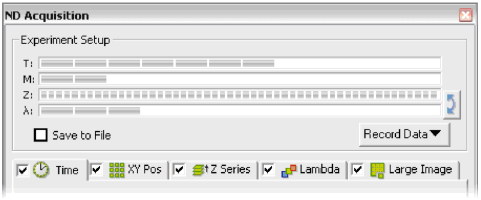
\includegraphics[scale=.70]{img/CAP26D.png}
 \caption{\small{Menu ND Acquisition per l'acquisizione in 6D.}}
 \label{fig:6D}
\end{figure}

Nel menu a tendina ``Time'' si impostano i parametri per l'\textit{acquisizione in time-lapse}, dove è possibile creare filmati in formato AVI. 
Via software si può impostare ogni quanto acquisire le immagini, da qualche $ms$ a qualche ora, tenendo presente che non è possibile acquisire le immagini ad intervalli temporali minori del tempo di esposizione settato per la telecamera. 
Le immagini vengono salvate in un file unico da cui è possibile estrarre solo alcuni fotogrammi o selezionare solo alcuni intervalli di tempo per produrre successivamente dei filmati separati, sempre in formato AVI. 
È inoltre possibile impostare diverse fasi di lavoro, salvate in file separati, e decidere per ciascuna fase il rate temporale di acquisizione e la durata totale dell'osservazione. 
La tendina ``XY Pos'' permette invece di impostare l'\textit{acquisizione in multi-point}, in cui si possono memorizzare varie posizioni (x, y, z), così da poter osservare più di un campo di vista all'interno del campione. 
Nel menu a tendina ``Z Series'' si imposta l'\textit{acquisizione in z-serie} che permette di acquisire immagini a diversi piani di fuoco e di visualizzarle poi in modalità tridimensionale, sfruttando un apposito algoritmo di deconvoluzione che elimina in parte i segnali fuori fuoco.
Nella tendina corrispondente al tasto ``Lambda'' si imposta l'\textit{acquisizione in multichannel}, ovvero si seleziona il filtro da utilizzare nella determinata sequenza spazio-temporale. 
Questo menu è particolarmente utile nel caso in cui si vogliano utilizzare più fluorofori per marcare diverse componenti del campione oppure nel caso in cui si vogliano acquisire immagini sia in campo chiaro che in fluorescenza. 
Nel menu ``Large Image'' si imposta l'\textit{acquisizione di immagini consecutive} che ricoprano un'area del campione stabilita dall'utente.
Inoltre, all'interno di ogni tendina è possibile settare ulteriori impostazioni, come per esempio decidere quando aprire e chiudere lo shutter e quando accendere o spegnere la luce usata in trasmissione.
Tuttavia, nel software sono presenti menu separati, oltre a quello per la misura in 6D, che permettono di eseguire solo un tipo alla volta di queste sequenze di acquisizione e menu che invece consentono di creare più fasi di sequenze 6D.

Bisogna notare che Nis-Element 3.1 è un software versatile non solo per quanto riguarda la fase di acquisizione delle immagini, ma anche per la parte di gestione e di elaborazione di quelle acquisite. 
Esso possiede infatti dei moduli che permettono una vasta gamma di operazioni di misura sulle immagini (\figurename~\ref{fig:dist}), come quantificare distanze, aree, perimetri e angoli, e operazioni di elaborazione (\figurename~\ref{fig:elab}), come l'aumento del contrasto, il rilevamento di bordi, la sogliatura ed alcune operazioni morfologiche (es. erosione e dilatazione).

\begin{figure}
 \centering
 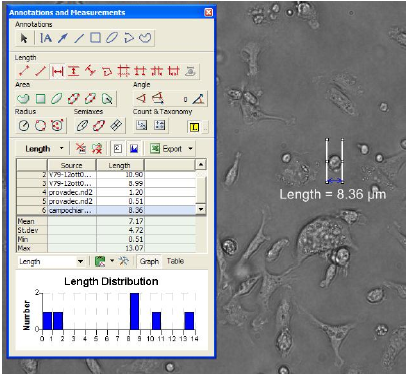
\includegraphics[scale=.60]{img/CAP2dist.png}
 \caption{\small{Esempio di utilizzo del software Nis-Element 3.1 per misure di distanza.}}
 \label{fig:dist}
\end{figure}

\begin{figure}
 \centering
 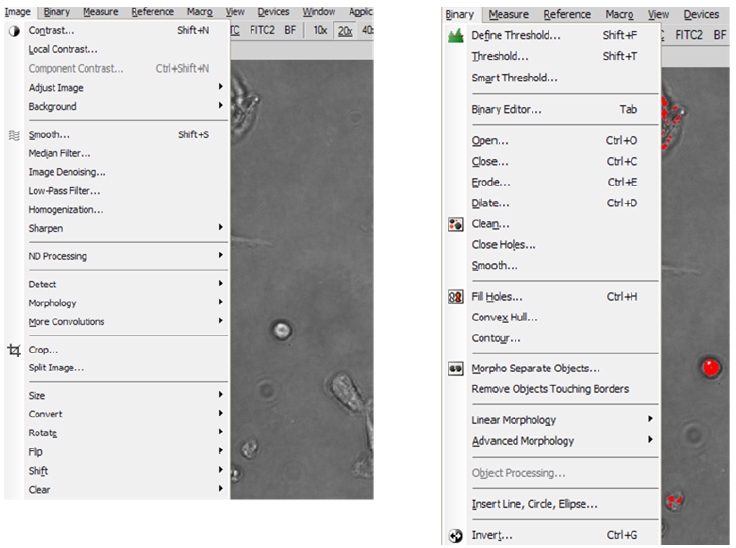
\includegraphics[scale=.40]{img/CAP2elab.png}
 \caption{\small{Panoramica di alcune operazioni di elaborazione di immagini previste dal software Nis-Element 3.1.}}
 \label{fig:elab}
\end{figure}


\section{Imperfezioni e difetti dell'immagine}

Nel campo dell'ottica, data la complessità dello studio geometrico del comportamento delle lenti, spesso ci si limita ad una trattazione basata sulla cosiddetta \textit{approssimazione di Gauss} \cite{difetti}. 
Questa teoria, detta anche ``teoria delle lenti sottili'' o ``ottica parassiale'', è applicabile per sistemi ottici ideali, ossia sistemi che soddisfano tali richieste:

\begin{itemize}
\item lenti di spessore trascurabile;

\item raggi incidenti parassiali, quindi molto prossimi all'asse della lente, e poco inclinati sull'asse, cosicchè tutti gli angoli da essi formati (es. angoli di incidenza, di apertura e di campo) siano piccoli, tali da approssimare $sin\theta \sim tan\theta$;

\item radiazione monocromatica;

\item onde sferiche o, nel caso in cui il loro raggio di curvatura  sia molto grande, piane.
\end{itemize}

Il risultato di tali ipotesi semplificative è che le immagini godono anch'esse di proprietà ideali, quali:

\begin{itemize}
\item l'immagine di un oggetto esteso, piano e perpendicolare all'asse è geometricamente simile all'oggetto e a sua volta piana e perpendicolare all'asse;

\item l'immagine di un oggetto privo di dimensioni, cioè di un punto, è ancora un punto;

\item i valori dell'ingrandimento, della focale e la posizione dei punti principali sono indipendenti dalle dimensioni dell'oggetto, dall'inclinazione dei raggi sull'asse e dalle lunghezze d'onda interessate;

\item il contrasto nell'immagine risulta uguale a quello nell'oggetto.
\end{itemize}

Ossia, sulla base dell'approssimazione di Gauss si otterrebbero immagini piane, non deformate e con risoluzione infinita, in quanto ogni punto dell'oggetto avrebbe il suo corrispondente nell'immagine e si potrebbero ritrovare in quest'ultima strutture e dettagli dell'oggetto piccoli quanto si vuole, con contrasto immutato (fino ai limiti di risoluzione del rivelatore).
Tuttavia sussistono tre cause principali di deviazione dello stato reale da quello ideale, e quindi dell'immagine effettivamente osservata da quella prevista secondo tale teoria: cause geometriche, fisiche e tecniche.
Tutte queste degradano l'immagine in vari modi, riducendone la qualità e limitando le possibilità di ottenere risultati quantitativi non distorti senza effettuare delle correzioni appropriate.

\subsection{Cause geometriche}

Quando si considerano sistemi reali di lenti spesse, con angoli di campo e di apertura non trascurabili e radiazione policromatica, risultano essere molto rilevanti per la formazione dell'immagine anche gli effetti rifrattivi sulle interfacce di riferimento (superficie aria-vetro o vetro-vetro).
Le differenze dall'immagine ideale causate da tale classe di deviazioni dalle condizioni ideali dell'ottica di Gauss sono globalmente indicate con il termine di \textit{aberrazioni}.

Il loro effetto globale è la produzione, per ogni punto oggetto, di un'immagine allargata, detta ``cerchio di confusione'', di forma e profilo fotometrico assai variabile. 
Tale cerchio danneggia sia la risoluzione dell'immagine che il microcontrasto, dove con tale termine si intende l'andamento fotometrico dell'immagine di un oggetto in cui una zona buia ed una luminosa sono separate da una linea netta, senza transizioni. 
Infatti, a causa della presenza del cerchio di confusione il passaggio chiaroscuro all'interno dell'immagine non è più rappresentabile con una curva a gradino, bensì avente pendenza più o meno regolare, comportando perciò una minor definizione (o nitidezza) dell'immagine stessa.

Le aberrazioni del punto possono essere di diverso tipo:
\begin{enumerate}
 \item aberrazione cromatica;
 \item aberrazione sferica;
 \item coma;
 \item astigmatismo;
 \item distorsione.
\end{enumerate}


\subsubsection*{Aberrazione cromatica}
L'aberrazione cromatica è legata alla lunghezza d'onda della radiazione osservata e perciò risulta assente per radiazione di tipo monocromatico. 
Ai fini della microscopia a fluorescenza, l'aberrazione cromatica risulta essere non trascurabile all'aumentare del numero di fluorofori differenti utilizzati all'interno del campione.

\begin{figure}
 \centering
 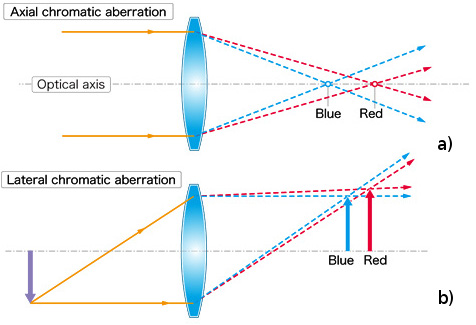
\includegraphics[scale=.60]{img/CAP2ac.jpg}
 \caption{\small{Formazione dell'aberrazione cromatica longitudinale (caso a) e trasversale (caso b).}}
 \label{fig:ac}
\end{figure}

Per la comprensione di tale fenomeno si supponga di utilizzare radiazione bianca per la formazione dell'immagine, così da disporre di un intero spettro continuo entro il range del visibile, ossia circa [400-800] nm. Ad ognuna delle lunghezze d'onda $\lambda$ interne a tale intervallo sarà associato un determinato indice di rifrazione $n$, secondo la legge di Cauchy \cite{nigro}:
$$n(\lambda) = A + \frac{B}{\lambda ^2}$$
dove A e B sono costanti dipendenti dal mezzo in esame.
Questo comporta un diverso angolo di deviazione, angolo tra la direzione entrante ed uscente del raggio, dato che, tramite costruzione geometrica, risulta direttamente proporzionale all'indice stesso.

Tale variazione dell'angolo di dispersione, quindi della focale, al variare della lunghezza d'onda provoca una variazione della coniugata immagine, dando origine alla cosiddetta \textit{aberrazione cromatica assiale o longitudinale}. 
Per tale effetto, un oggetto che emette o è attraversato da luce bianca fornisce una serie di sue immagini di differente colore, a diversa distanza dalla lente: la distanza massima si avrà per le lunghezze d'onda maggiori (parte rossa del visibile) poiché corrispondenti ad indice di rifrazione minore e quindi focale maggiore (\figurename~\ref{fig:ac}/a). 
Si ha dunque una successione di immagini corrispondenti ai valori di lunghezza d'onda presenti, detta ``spettro primario'' e l'immagine risultante appare quindi circondata da aloni colorati (\figurename~\ref{fig:aca}).

\begin{figure}
 \centering
 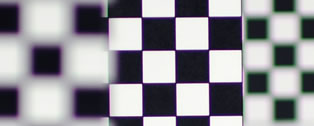
\includegraphics[scale=.88]{img/CAP2aca.jpg}
 \caption{\small{Esempio di aberrazione cromatica assiale.}}
 \label{fig:aca}
\end{figure}

Supponiamo a questo punto di ignorare o di avere corretto la cromatica assiale e quindi che la posizione focale dell'immagine sia unica per tutto lo spettro.
Ciò nonostante, la dispersione dell'indice di rifrazione e della focale portano ad un diverso ingrandimento per ogni valore di lunghezza d'onda (\figurename~\ref{fig:ac}/b). 
Questo significa, sempre operando in luce bianca, che le infinite immagini possono anche giacere sullo stesso piano, ma hanno diverse dimensioni (\figurename~\ref{fig:acl}). 
Tale effetto viene definito con il nome di \textit{aberrazione cromatica laterale o trasversale}.
In tal caso gli aloni non esistono al centro del campo e crescono di larghezza all'aumentare della distanza dall'asse, cioè del campo stesso.

\begin{figure}
 \centering
 
\includegraphics[scale=.40]{img/CAP2acl.jpg}
 \caption{\small{Aberrazione cromatica laterale della Luna.}}
 \label{fig:acl}
\end{figure}

Per ridurre la cromatica assiale si possono combinare vetri con diverso potere dispersivo, così da ottenere sistemi convergenti o divergenti in cui i valori di focale e di immagine coniugata coincidono per due lunghezze d'onda agli estremi dello spettro visibile. 
In ordine del grado di complessità crescente e del numero di lenti utilizzate nel sistema, si hanno le cosiddette correzioni acromatiche ed apocromatiche, associate ai corrispondenti obiettivi acromatici ed apocromatici. 
Inoltre il diametro del suo cerchio di confusione diminuisce chiudendo il diaframma d'apertura. 
Tale aberrazione dipende molto dalla combinazione dei sistemi ottici (obiettivo, oculare e sistemi intermedi) e può essere ridotta tramite l'uso di filtri. 
Per quanto riguarda la cromatica laterale, la larghezza delle frange colorate prodotte non dipende dall'apertura del diaframma.
Ancor più della longitudinale, questa cromatica è sensibile all'accoppiamento obiettivo-oculare, alla presenza di sistemi intermedi ed all'uso di filtri.

\subsubsection*{Aberrazione sferica}
L'aberrazione sferica è un'aberrazione del punto di tipo acromatico, ossia presente anche con radiazione monocromatica, pur essendo il suo andamento legato al valore della lunghezza d'onda in gioco.
L'aberrazione sferica è una variazione della focale e quindi della posizione dell'immagine al variare dell'apertura. 

\begin{figure}
 \centering
 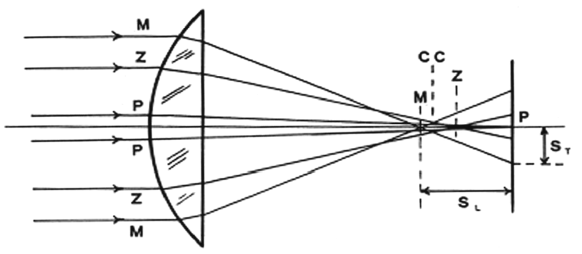
\includegraphics[scale=.50]{img/CAP2as.png}
 \caption{\small{Formazione dell'aberrazione sferica.}}
 \label{fig:as}
\end{figure}

La \figurename~\ref{fig:as} illustra il fenomeno nel caso particolare di distanza infinita del punto dalla lente: per uno stesso punto oggetto si hanno diverse immagini a diversa distanza dalla lente al variare dell'apertura, ossia dell'inclinazione, degli infiniti raggi convergenti nell'immagine.
Si identificano un fuoco ``parassiale'' P formato alla minima apertura, un fuoco ``marginale'' M alla massima apertura ed uno ``zonale'' Z formato da raggi appartenenti ad una regione intermedia.
Qualunque dei fuochi sopra citati si scelga come migliore immagine, esso sarà sempre circondato da un alone dovuto ai raggi che convergono in un fuoco più vicino o più lontano (\figurename~\ref{fig:sfer}). Questo alone è sempre presente e si può solamente cercare di minimizzarlo. 

\begin{figure}
 \centering
 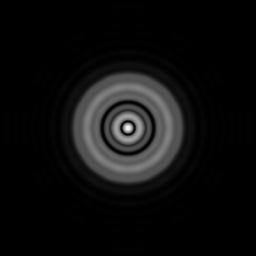
\includegraphics[scale=.55]{img/CAP2sfer.jpg}
 \caption{\small{Esempio di aberrazione sferica su un punto oggetto.}}
 \label{fig:sfer}
\end{figure}

L'inviluppo di tutti i raggi appartenenti a tutte le zone della lente costituisce una figura caratteristica, detta ``caustica'', che, sezionata con un piano perpendicolare all'asse, mostra sempre una figura circolare, mai un punto.
\'E proprio la caustica che rappresenta il cerchio di confusione dovuto all'aberrazione sferica e si cercherà sempre il cerchio di minima confusione, (CC in \figurename~\ref{fig:as}), dato che tale figura si può minimizzare cercando il miglior fuoco, ma mai annullare.

Il termine ``sferica'' si riferisce al fatto che tale aberrazione è legata alla forma sferica delle superfici delle lenti usuali e perciò si può eliminare dando forme asferiche particolari, metodo utilizzato per collettori, condensatori e certi obbiettivi fotografici, oppure combinando lenti sferiche di forma ed indice diversi, metodo utilizzato nei microscopi. 
Un sistema corretto dall'aberrazione sferica si chiama aplanatico.

\subsubsection*{Coma}
La coma ha come radice etimologica i termini ``chioma'', ``cometa'', facendo riferimento al suo tipico aspetto, ancor più evidente se agente su piccoli oggetti (\figurename~\ref{fig:coma}).

\begin{figure}
 \centering
 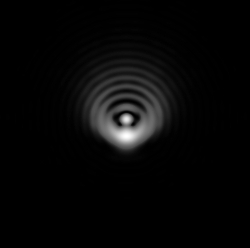
\includegraphics[scale=.55]{img/CAP2coma.jpg}
 \caption{\small{Esempio di coma su un punto oggetto.}}
 \label{fig:coma}
\end{figure}

Questa aberrazione acromatica è di tipo extra-assiale, così come la cromatica laterale, ossia non esiste sull'asse di un sistema centrato e cresce con l'aumentare del campo. 
Di conseguenza il suo cerchio di confusione non può essere circolare ma risulta allungato in senso radiale e presenta un punto molto luminoso che sfuma gradatamente in una larga coda.
Questo difetto ha origine quando l'oggetto osservato non è allineato con l'asse di osservazione.

In microscopia la coma si corregge facilmente scegliendo in modo opportuno la posizione del diaframma e la forma delle lenti, prestando attenzione al fatto che essa è assente in un sistema simmetrico col diaframma al centro.
Risulta ovvio che la coma in asse non può esistere, perciò se al centro del campo di un microscopio si osserva un residuo di coma in generale è indice che una o più lenti dell'obiettivo non sono centrate sull'asse comune.

\subsubsection*{Astigmatismo}
L'astigmatismo è un'aberrazione acromatica, extra-assiale che crea un'immagine sdoppiata e deformata di ogni punto oggetto (\figurename~\ref{fig:astigmatismo}). In tal caso, il fascio di raggi che convergono nell'immagine di un punto oggetto non si raccoglie attorno ad una zona circolare, bensì attorno ad un segmento tangenziale, detto ``focale astigmatica''.
Questo è dovuto ad un differente fuoco per angoli di rotazione intorno all'asse ottico.
Un fascio conico a sezione circolare viene quindi deformato in uno non circolare in seguito alla diversa focale che i raggi hanno.

\begin{figure}
 \centering
 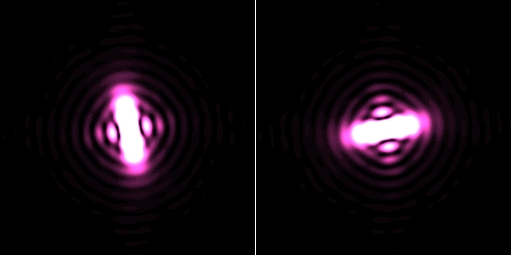
\includegraphics[scale=.50]{img/CAP2astig.jpg}
 \caption{\small{Esempi di astigmatismo su un punto oggetto.}}
 \label{fig:astigmatismo}
\end{figure}

L'astigmatismo, come la coma, è nullo sull'asse e cresce col campo. 
Se nell'uso pratico si riscontra astigmatismo anche al centro del campo allora le cause possono essere varie: inclinazione di qualche prisma o di qualche lente rispetto all'asse, errore di centratura o errore nella forma di qualche lente.
Tuttavia modificando la messa a fuoco del microscopio, si evince una grande differenza tra la figura della coma e dell'astigmatismo nell'immagine di un punto oggetto: la prima si può allargare ma conserva la sua forma, con la coda che resta diretta radialmente, mentre la seconda si allunga in direzione da radiale a tangenziale o viceversa. 

Per la correzione di tale aberrazione bisogna tener conto che essa è influenzata, più che dalla forma delle lenti, dalla posizione del diaframma e dal numero di lenti interposte, dato che una lente divergente mostra un astigmatismo di segno opposto di una convergente, da cui l'utilità di porne varie in successione. 
Un sistema corretto da astigmatismo si chiama genericamente ``anastigmatico''. 

\subsubsection*{Distorsione}
La distorsione consiste in una variazione dell'ingrandimento trasversale con la distanza dall'asse, per cui l'immagine di un oggetto esteso piano non gli è simile. 
Se l'ingrandimento cresce col campo, cioè con la distanza del punto dall'asse, allora l'oggetto sembra dilatarsi verso la periferia e si parla di distorsione positiva o ``a cuscinetto''; viceversa, se l'ingrandimento diminuisce al crescere del campo allora l'oggetto sembra contrarsi e si ha la cosiddetta distorsione negativa o ``a barilotto'' (\figurename~\ref{fig:distorsione}).

\begin{figure}
 \centering
 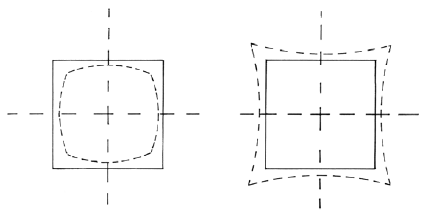
\includegraphics[scale=.65]{img/CAP2disto.png}
 \caption{\small{Distorsione a barilotto (sinistra) e a cuscinetto (destra) di un oggetto quadrato.}}
 \label{fig:distorsione}
\end{figure}

La distorsione di una lente sottile è in genere trascurabile, non è invece così per le lenti spesse: una lente spessa convergente tende a mostrare una distorsione positiva, se invece divergente la mostra negativa.
Tuttavia in microscopia la distorsione disturba i fini dell'esperimento solo quando si debbono eseguire misure di superficie o di lunghezza sull'oggetto, ma in genere essa è assai contenuta ed in prevalenza data dall'oculare poichè quella dell'obbiettivo non supera in genere l'1\%.
Un sistema corretto da distorsione e curvatura di campo si dice ortoscopico.


\subsection {Cause fisiche}

Finora abbiamo esaminato molti fenomeni ottici, che si verificano nel microscopio, servendoci di un approccio per lo più di natura geometrica e si è visto in tale contesto che, dato un punto oggetto, un sistema ottico reale non produce mai un'immagine puntiforme, se non altro a causa delle aberrazioni del punto.
Supponendo ora di operare in un sistema ideale, in cui siano assenti sia le aberrazioni che i difetti costruttivi, ebbene nuovamente non riusciremo ad ottenere da esso un'immagine puntiforme. 
Ciò è dovuto al fatto che la radiazione elettromagnetica non si può trattare sempre come se costituita da semplici ``raggi'', ossia rette di propagazione che obbediscono solo a leggi geometriche, bensì è necessario tenere conto della sua natura ondulatoria.
Una tipica conseguenza che si evince da tale approccio fisico alla propagazione della radiazione è la generazione di effetti diffrattivi.

Per comprendere tale fenomeno consideriamo una sorgente puntiforme Q, posta davanti ad uno schermo avente una fenditura circolare P, con una lente convergente L posta a ridosso dell'apertura, che crea sullo schermo S l'immagine Q' dell'oggetto Q (\figurename~\ref{fig:diff}).
Si noti l'evidente analogia che intercorre tra la fenditura P ed un diaframma d'apertura per la lente L.

\begin{figure}
 \centering
 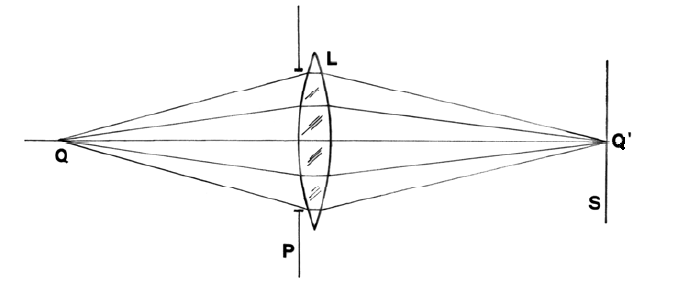
\includegraphics[scale=.55]{img/CAP2diff.png}
 \caption{\small{Schema del sistema fenditura-lente convergente per la formazione della figura di diffrazione.}}
 \label{fig:diff}
\end{figure}

Supponendo che la lente sia stata corretta da ogni tipo di aberrazione, il cerchio di confusione è previsto con raggio nullo. 
In realtà ciò che si osserva in Q' è una figura caratteristica, detta \textit{figura di diffrazione}, o anche ``figura di Airy'' o ``centrica'', avente l'aspetto tipico mostrato dalla \figurename~\ref{fig:diff2}: un disco centrale di massima intensità con orli sfumati (``disco di Airy''), circondato da una successione di anelli concentrici scuri e chiari, sempre sfumati e di intensità decrescente.

\begin{figure}
 \centering
 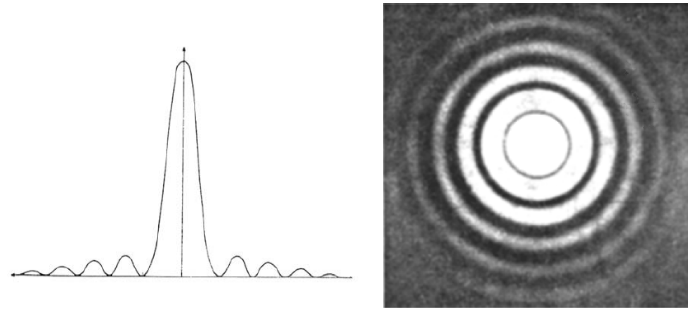
\includegraphics[scale=.55]{img/CAP2diff2.png}
 \caption{\small{Profilo fotometrico della centrica (sinistra) e figura di Airy (destra).}}
 \label{fig:diff2}
\end{figure}

Detta $NA$ l'apertura numerica della lente L e $\lambda$ la lunghezza d'onda dell'onda incidente, i valori del raggio dell'ennesimo anello chiaro sono:
$$r_n = k_n \frac{\lambda}{NA} $$
dove $k_n$ vale 0.61, 1.12 e 1.62 rispettivamente per il primo (disco di Airy), secondo e terzo anello chiaro.
\'E inutile andare oltre poiché gli anelli successivi sono troppo poco intensi per poter essere osservati, dato che l'intensità decresce molto rapidamente nelle varie zone della centrica. 
Infatti per il  disco di Airy l'energia è l'84\% di quella totale e per i successivi anelli: 7,1\%, 2,8\% e 1,5\%.

Dunque, un sistema ottico ideale, anche in assenza di aberrazioni, non dà un'immagine puntiforme di un punto oggetto, ma nuovamente una sorta di cerchio di confusione, questa volta non dovuto a fenomeni geometrici, quali la rifrazione, ma a fenomeni ondulatori, cioè alla diffrazione.

L'effetto diffrattivo, al contrario delle aberrazioni, è una proprietà intrinseca alla natura fisica del fenomeno in esame e perciò è molto più difficile poter limitare i difetti da esso apportati sull'immagine. 
Tuttavia, in alcuni casi, esso può venire attenuato tramite algoritmi applicati in una fase post-acquisizione sull'immagine desiderata, come per esempio con il cosiddetto \textit{algoritmo di deconvoluzione}.
Questa  tecnica inizialmente nacque con lo scopo di rimuovere le sfocature caratteristiche di un sistema fuori fuoco che contaminavano le immagini di una vasta gamma di microscopi \cite{decon}. 

\begin{figure}[h]
 \centering
 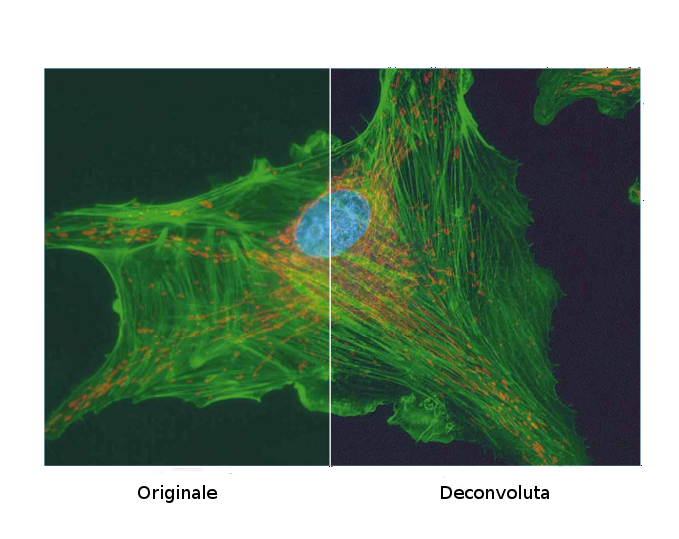
\includegraphics[scale=.60]{img/CAP2decon.png}
 \caption{\small{Immagine a fluorescenza di una cellula endoteliale di bovino. La regione a sinistra mostra l'immagine originale, quella a destra il risultato di un processo iterativo di deconvoluzione bidimensionale.}}
 \label{fig:decon}
\end{figure}

Un microscopio è in genere caratterizzato dalla sua ``Point Spread Function'' (PSF), una descrizione bidimensionale o tridimensionale di come un singolo punto luce venga trasformato dallo strumento e mostrato all'utilizzatore. 
La PSF è determinata dalla combinazione delle caratteristiche ottiche del campione, del vetrino, delle lenti dell'obiettivo e della lunghezza d'onda usata; per esempio un microscopio confocale ha tipicamente una PSF che assomiglia ad un ellissoide posto nella direzione assiale.
Un oggetto arbitrario può essere pensato come insieme di punti luce posti in diverse posizioni, con differenti intensità. 
Quindi, l'immagine osservata dall'utilizzatore può essere descritta come una sovrapposizione di varie PSF, ciascuna nella posizione del corrispondente punto luce all'interno del campione, con intensità opportunatamente scalata.
Matematicamente tale operazione è detta ``convoluzione'', perciò, invece che vedere un'immagine pulita, si osserva, a causa della sovrapposizione delle PSF, una sfocatura che copre le caratteristiche di interesse. 
Di conseguenza l'immagine ottenuta dal microscopio non è una rappresentazione fedele dell'oggetto in esame, bensì una semplice rappresentazione di esso.
L'operazione necessaria per correggere questa ``sfocatura'' è detta deconvoluzione, in quanto corrisponde all'operazione inversa della convoluzione che ha dato origine all'immagine.
Lo scopo della deconvoluzione è proprio utilizzare la rielaborazione via software per invertire tale processo e ripristinare l'immagine fedele dell'oggetto in esame. 
Questo particolare algoritmo sta diventando negli ultimi anni parte integrante della microscopia digitale poiché, come si evince dalla \figurename~\ref{fig:decon}, è in grado di produrre immagini rielaborate con maggior risoluzione, miglior contrasto e rapporto segnale-rumore più elevato.

\subsection {Cause tecniche} 

L'immagine acquisita con il microscopio può essere affetta da difetti non solo di natura fisica-geometrica ma anche di origine tecnica-strumentale. 
In linea di principio si tratta di difetti eliminabili con opportuni accorgimenti tecnici, generalmente con un certo aggravio di costi di produzione e manutenzione.

Essi possono essere legati ad una imprecisa lavorazione dei materiali presenti all'interno del microscopio, come per esempio: irregolarità delle superfici, difetti nell'omogeneità dei materiali trasparenti, luce diffusa sulle pareti o sulle montature delle lenti, difetti di montaggio e di centratura, errori di messa a fuoco e mancata pulizia.

D'altra parte si può trattare anche di difetti intrinseci alla misura stessa, come ad esempio la presenza di una fluorescenza residua di sfondo e la non omogeneità del fascio. 
Entrambe sono connesse alla luce di eccitazione utilizzata durante l'esperimento: la prima inserisce un offset di luminosità nel background dell'immagine, mentre la seconda crea immagini con, a priori, intensità differente a seconda della posizione del pixel preso in esame, causate da un fascio di radiazione di per sé non omogeneo.

